\documentclass[12pt,english]{scrartcl}

\usepackage{amsmath,amssymb}
%\usepackage[amssymb]{SIunits}
\usepackage{babel}
\usepackage[latin1]{inputenc}
\usepackage{graphicx}
\usepackage{color}
\usepackage{url}


\begin{document}

\begin{center}
\textbf{\begin{LARGE}KOGW-PM-KNP:\\ \vspace{3mm} Tutorial 11 - The El Greco Fallacy in Perception Research
\end{LARGE}}
\end{center}

This tutorial deals with a particular kind of cognitive bias. The paper by Firestone \& Scholl (2016) introduces a certain kind of bias and suggests that the rationale of several paradigms in perception research are contaminated by that very bias. Please read the paper critically. Answer the following questions which should help you to evaluate their findings. Please work in pairs. 
%  
% \begin{figure}[htbp]
% \begin{center}
% 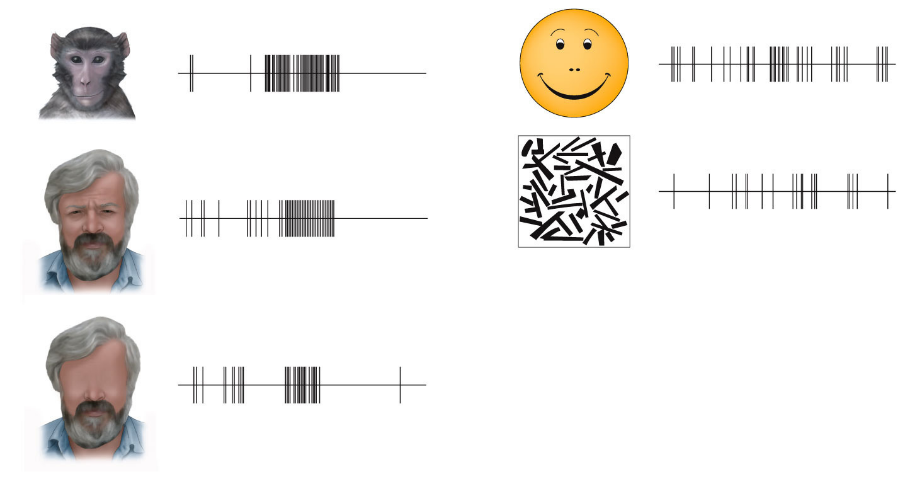
\includegraphics[width = 0.8\textwidth]{IT_cell.png}
% \end{center}
% \caption{
% \label{fig:IT_cell}}
% \end{figure}

\begin{enumerate}
 \item What does the \textit{cognitively impenetrability} hypothesis of perception say? Name one type of evidence that supports the hypothesis.

 \color{blue}
 \begin{itemize}
 \item processes responsible for computing basic visual attributes such as lightness of a colored patch proceed without any direct influence from higher-level cognitive states
 \item persistence of visual illusions despite conflicting knowledge about the visual input
 \item susceptibility to magic tricks despite better knowledge
 \end{itemize}
  \color{black}

 \item Explain the El Greco Fallacy with the help of a sketch that illustrates stimuli in the outside world, how they are perceived and how they would be painted.

 \color{blue}
 \begin{itemize}
 \item El Greco's figures were oddly elongated
 \item suffered from severe astigmatism and experienced a stretched-out world
 \item painted what he saw
 \item problem - figures painted by him and looking stretched to people with normal vision should look even more stretched out to him
 \end{itemize}
  \color{black}

 \item Describe the original finding that the authors wanted to replicate in their Experiment 1.

 \color{blue}
 \begin{itemize}
 \item perceived aperture looks narrower when observers carry a lenghty rod across their body
\end{itemize}
  \color{black}

 \item Describe the procedure and results of experiment 1.

 \color{blue}
 \begin{itemize}
 \item 2 conditions: with (114.3cm) and without rod
 \item estimate the width of an aperture (2.5m away) by having the experimenter (2m away) drewing out measurement tape until it visually matches the aperture's width
 \item aperture widths: 76.2, 88.9, 101.6, 114.3, 127, 139.7, 152.4; 5 repeats each
 \item[]
 \item subjects holding the rod judged the aperture to be narrower: 105 vs. 112cm
\end{itemize}
  \color{black}


 \item Describe the procedure and logic underlying experiment 2. What were the results?
 
 \color{blue}
 \begin{itemize}
 \item identical to Experiment 1 except that the 'measuring device' was itself an adjustable aperture = matching aperture 
 \item if holding a rod really does perceptually compress apertures then this variant should fail to produce the effect

 \item[]
 \item subjects holding the rod judged the aperture to be narrower: 106 vs. 111cm
\end{itemize}
  \color{black}


 \item What type of effect do the experimenters test in Experiment 3? Describe the procedure and the results.

 \color{blue}
 \begin{itemize}
 \item experimental demand characteristic 
 \item cover story: purpose of rod was to improve their balance, testing the effect of rods of different sizes
 \item[]
 \item subjects holding the rod judged the aperture like those in Exp 1 and 1: 111cm
 \item supports nonperceptual explanation for the aperture-width effects in terms of demand characteristics
\end{itemize}
  \color{black}

\item What do the authors suggest as a reason for why it has been difficult to provide evidence for the absence of top-down effects. 
 \color{blue}
 \begin{itemize}
 \item reluctance to report null effects 
\end{itemize}
  \color{black}
 

\item Do you perceive any problems with the research reported in the article - with respect to methodology, reasoning, ... etc.? 
 \color{blue}
 \begin{itemize}
 \item results averaged across aperture width
 \item difference between test and match aperture distances
 \item experimenter not naive wrt purpose of the experiment 
\end{itemize}
  \color{black}

\end{enumerate}

\end{document}
